\section{Teoria dell'Apprendimento: Agenti capaci di apprendere}
    Il vantaggio di un agente capace di apprendere è che lavora in un ambiente inizialmente sconosciuto e diventa più bravo col tempo.
    
    Questo tipo di agenti hanno quattro componenti principali:
    \begin{itemize}
        \item \textbf{Elemento di apprendimento:} Responsabile del miglioramento interno.
        
        \item \textbf{Elemento esecutivo:} L'elemento responsabile delle azioni esterne. Questo è ciò che fino ad ora abbiamo considerato come agente.
        
        \item \textbf{Elemento critico:} L'elemento responsabile di fornire feedback sulle prestazioni attuali dell'agente. Sulla base di queste informazioni l'elemento di apprendimento potrebbe prendere azione per modificare il modo di ragionare dell'agente.
        
        \item \textbf{Generatore di problemi:} Questo elemento è responsabile di suggerire azioni che portino l'agente a fare esperienze nuove e significative.
    \end{itemize}
    
    Nella nostra accezione, l'apprendimento consta nel miglioramento di un agente intelligente in un certo ambiente, ossia \textbf{migliorare} con l'\textbf{esperienza} nell'esecuzione di un \textbf{task}.
    
    Il \textbf{machine learning} ci permette di imparare dai dati, e infatti in questo corso parliamo di algoritmi che vanno oltre la classica concezione di eseguire una serie di istruzioni, ma saranno in grado di prendere \textbf{decisioni data-driven}.
    
    Nonostante gli algoritmi di machine learning abbiano una storia molto lunga, sono esplosi negli ultimi anni a causa di strumenti elaborativi più adeguati e una grande disponibilità di dati.
    
    Questi algoritmi si suddividono principalmente in:
    \begin{itemize}
        \item \textbf{Apprendimento supervisionato:} Gli elementi da cui l'agente deve apprendere, ossia i dati, sono \textit{etichettati}, e le etichette definiscono anche la variabile dipendente, ciò che l'agente dovrà apprendere.
        
        \item \textbf{Apprendimento non supervisionato:} In questo caso l'agente apprende a partire da dati \textit{non etichettati}, e quindi sarà in grado di imparare senza conoscere la variabile dipendente.
    \end{itemize}
    
    Oltre a queste due categorie ci sono altre categorie, come l'apprendimento semi-supervisionato, in cui alcuni dati sono etichettati e altri no, e quello per rinforzo, in cui l'agente esegue una sequenza di azioni, al termine delle quali ottiene una ricompensa (questo è simile al metodo di apprendimento Pavloviano).
    
    Oltre alla classificazione degli algoritmi, possiamo suddividere i problemi in base all'output che vogliamo ottenere:
    \begin{itemize}
        \item \textbf{Classificazione:} Abbiamo delle etichette discrete e vogliamo assegnarne una all'oggetto in esame.
        
        \item \textbf{Regressione:} Range di valori continui da assegnare all'oggetto in esame.
        
        \item \textbf{Clustering:} Una suddivisione dei dati in gruppi.
    \end{itemize}
    
    Possiamo andare a migliorare e semplificare il problema tramite tecniche come la \textbf{riduzione della dimensionalità}, che ci permette di ridurre le caratteristiche significative e di eliminare quelle ridondanti, e il \textbf{mining di associazioni}, che ci permette di identificare pattern comuni in una serie di transazioni. Quest'ultimo è in pratica il \textit{market basket analysis}.
    
    Ovviamente non c'è un algoritmo migliore, ma dipende dalle risorse che abbiamo a disposizione e dal problema che dobbiamo trattare. Ci possiamo affidare al \textbf{metodo empirico} per scegliere l'algoritmo migliore fra quelli che la teoria ci dice essere utilizzabili. Possiamo costruire diversi modelli, procedere alla \textbf{misura dell'errore} per ognuno di essi e scegliere quello con la misura d'errore minore.
    
    \subsection{Errore, Bias e Varianza}
        L'\textbf{errore}, o residuo, è la differenza fra il valore stimato e quello reale.
        
        Introduciamo il concetto di \textit{errore irriducibile}, ossia quell'errore che dipende da una variabile intrinseca del problema. Pensiamo al calcolare l'altezza di una persona: anche persone identiche per molte altre variabili, potrebbero avere altezze diverse. Il nostro scopo è quindi avvicinarci ai dati reali nel margine dell'errore irriducibile.
        
        Il modello ha un certo \textbf{bias} se quando viene addestrato su diversi dataset, restituisce un output sistematicamente \textit{sbagliato}. Questo avviene quando il modello deve fare troppe assunzioni. Questa situazione viene detta anche \textit{underfitting}.
        
        Parliamo di \textbf{varianza} quando il modello restituisce un output sistematicamente \textit{diverso} quando viene addestrato su dataset diversi. Un'alta varianza è anche detta \textit{overfitting}.
        
        L'obiettivo sarebbe dunque rendere nulli bias e varianza. Tuttavia questi sono inversamente proporzionali, e quindi è necessario trovare un compromesso fra i due, che permetta al modello di essere abbastanza flessibile pur sapendo come comportarsi su dati mai visti.
        
    \subsubsection{Underfitting e Overfitting}
        Un modello soggetto a \textbf{underfitting} non sa imparare dai dati, soprattutto se essi sono complessi. Un modello del genere non saprà come rispondere a un nuovo set di dati in quanto non avrà imparato abbastanza dai dati di training.
        
        Un modello che soffre di \textbf{overfitting} avrà il problema opposto, ossia si abituerà troppo ai dati di training e non riuscirà a risolvere problemi anche solo leggermente diversi, in quanto non riesce a estrarre generalità da ciò che impara. Possiamo concettualmente paragonarlo a uno studente che studia a memoria.
        
\section{Dati}
    L'intelligenza artificiale è una scienza che richiede moltissimi dati.
    
    In questo contesto l'\textbf{ingegneria dei dati} è l'insieme di tecniche e algoritmi che permettono l'estrazione, l'analisi e il trattamento di dati allo scopo di renderli fruibili ad altre tecniche o algoritmi di data analytics. Questo è certamente importante ma dipende molto anche dalla \textbf{qualità dei dati}, la quale indica l'accuratezza, la coerenza e la completezza dei dati. Partendo da dati fallati, difficilmente possiamo ottenere buoni risultati, a prescindere da quanto li trattiamo.
    
    La \textbf{data governance} infine gestisce la disponibilità, usabilità e integrità dei dati, ed è basata su standard interni di un'organizzazione.
    
    Quando un modello è capace di lavorare bene in fase di addestramento ma non in fase di rilascio, potremmo avere un porblema di \textbf{data leakage}. Un \textit{leaky predictor} è infatti un dato che ci aiuta a fare una previsione corretta, ma che non necessariamente è disponibile in fase di rilascio. 
    
    \subsection{Tipologie di dati}
        Non tutti i dati sono creati uguali: sono sicuramente tutti definiti come elementi di cui si dispone per risolvere un dato problema, ma ne esistono diversi tipi:
        \begin{itemize}
            \item \textbf{Dati strutturati:} Sono dati tabulari le cui righe e colonne sono ben definite e il cui formato è molto rigido. Includono basi di dati, file XML, JSON, etc.
            
            \item \textbf{Dati non strutturati:} Sono perlopiù dati che non ricadono nella precedente categoria. Possono essere file audio, testuali (per i quali esiste un'intera branca chiamata Natural Language Processing), etc. Sono i più difficili da estrarre e trattare in quanto servono strumenti ad hoc.
            
            \item \textbf{Dati semi-strutturati:} Questi sono dati che hanno un formato sempre uguale ma la cui struttura potrebbe variare: per esempio dati tabulari potrebbero avere elementi mancanti o parti espresse in maniera non strutturata.
        \end{itemize}
        
\section{Data Preparation}
    Questo include, in maniera sequenziale, \textbf{Data Cleaning}, \textbf{Feature Scaling}, \textbf{Feature Selection} e \textbf{Data Balancing}.
    
    \subsection{Data Cleaning}
        È il processo di non danneggiare l'intero processo di machine learning a causa di dati mancanti o rumorosi. Possiamo ricorrere alla \textbf{data imputation}, che può stimare il valore dei dati mancanti a partire da quelli presenti o mitigare il problema causato da dati mancanti.
        
        Due soluzioni banali sono \textbf{scartare righe o colonne} con elementi mancanti. Questa soluzione rimuove il problema ed è raccomandabile, però non sempre è applicabile. Se abbiamo pochi dati con cui lavorare non possiamo permetterci tali scarti.
        
        Un altro metodo è l'\textbf{imputazione statistica}, che ricava il valore dei dati mancanti tramite semplici tecniche statistiche, come la media. Anche questa tecnica è semplice e veloce da applicare ma non applicabile su dati non numerici e inoltre non tiene conto dell'incertezza.
        
        Ovviamente non c'è una tecnica migliore in assoluto e dipende dal problema. Dobbiamo tenere presente la possibilità di usare più tecniche e/o di introdurre l'intervento umano, per esempio nella forma di deduzione.
        
        Questo per quanto riguarda i dati strutturati. Ovviamente per quelli non strutturati la cosa diventa ancora più difficile e specifica. Ogni problema potrebbe avere una soluzione diversa, si pensi per esempio ai problemi di NLP che variano da lingua a lingua in maniera significativa.
        
    \subsection{Feature scaling}
        Potremmo trovarci nel caso in cui due caratteristiche abbiano una distribuzione significativamente diversa, e questo può impattare le prestazioni di un machine learner, in quanto esso potrebbe sovrastimare o sottostimare l'importanza di una certa caratteristica.
        
        Un esempio palese è l'altezza di una persona espressa in centimetri, che è nell'ordine delle centinaia, e l'anno di nascita che è ha un intero ordine di grandezza in più.
        
        Definiamo come \textbf{feature scaling} l'insieme di tecniche che permettono di normalizzare o scalare l'insieme di valori di una caratteristica. Uno dei metodi più comuni è la \textit{min-max normalization}, mentre un'alternativa spesso considerata è quella della \textit{z-score normalization}, che prende in considerazione la distribuzione standard delle caratteristiche.
        
    \subsection{Feature selection}
        Il \textbf{feature engineering} è il processo di definire una serie di caratteristiche significative in base alla conoscenza del dominio. Questa fase è molto importante in quanto dà un senso a dati strutturati, ma soprattutto a dati non strutturati e semi-strutturati. È anche molto complesso in quanto è il processo che richiede maggiore creatività e conoscenza del dominio.
        
        La scelta di dati significativi porta a una \textit{maggiore flessibilità} del modello, e quindi a risultati buoni anche usando algoritmi sub ottimi (\textit{"More data beats clever algorithms, but better data beats more data"}). Aumentano anche la \textit{semplicità} del modello, la sua \textit{explainability} e le sue \textit{prestazioni}.
        
        Abbiamo diversi sotto-campi della feature engineering, fra cui feature extraction, feature construction e feature selection.
        
        I primi due differiscono poiché il primo punta a generare automaticamente dati dal problema, e infatti viene chiamata anche riduzione della dimensionalità siccome parte da un insieme più grande per estrarre solo alcune features, mentre la seconda punta alla costruzione di feature da parte del progettista. Infine la feature selection punta a selezionare le variabili più significative a partire da quelle a disposizione, e differisce dalla feature extraction in quanto quest'ultima parte dai dati grezzi e li converte in nuovi tipi di dati.
        
    \subsection{Data balancing}
        Molti dei problemi reali sono \textit{sbilanciati}. Pensiamo per esempio a tutti i problemi di carattere medico; ci interessa conoscere quando una malattia viene diagnosticata, ma un modello di machine learning non bilanciato saprà riconoscere solo gli elementi più popolosi nel dataset, e quindi riconoscere bene gli individui sani, di cui ci interessa relativamente poco.
        
        Le tecniche applicate per bilanciare il dataset sono principalmente due: \textit{undersampling} e \textit{oversampling}.
        
        Il primo rimuove casualmente istanze (righe) dal dataset, ma potrebbe andare a eliminare istanze importanti, oltre che ridurre troppo il numero di istanze.
        
        L'oversampling invece aggiunge casualmente istanze. Tuttavia semplicemente copiare istanze già esistenti potrebbe causare overfitting.
        
\section{Classificazione e Classificatori}
    La \textbf{classificazione} viene definita come un task in cui un classificatore deve predire il valore di una variabile dipendente partendo da una serie di istanze appartenenti a un training set per le quali questa variabile è conosciuta.
    
    I problemi di classificazione sono istanze di problemi di apprendimento supervisionato.
    
    Esistono diverse decine di classificatori basati sulla maniera in cui trattano i dati e apprendono, ma vedremo principalmente Naive Bayes e Decision Tree. Oltre ai classificatori di base esistono gli ensamble, i quali combinano i risultati di diversi classificatori di base.
    
    \subsection{Naive Bayes}
        l'algoritmo considera le caratteristiche della nuova istanza e clacola la probabilità che queste facciano parte di una determinata classe tramite il teorema di Bayes. Parliamo di algoritmo naive in quanto va a considerare le caratteristiche come indipendenti l'una dall'altra.
        
        La classificazione avviene secondo tre step:
        \begin{enumerate}
            \item \textbf{Calcolo delle probabilità di una classe:} Sono semplicemente le frequenze delle istanze che appartengono a ciascuna classe per il numero totale di istanze.
            
            \item \textbf{Calcolo della probabilità condizionata:} Si applica il teorema di Bayes.
            
            \item \textbf{Decisione:} Identificata nella classe che ottiene il valore di probabilità più alto.
        \end{enumerate}
        
    \subsection{Alberi decisionali}
        L'algoritmo mira a creare un albero in cui i nodi rappresentano un sotto-insieme delle caratteristiche e i cui archi rappresentano delle decisioni.
        
        Gli alberi decisionali sono utili per la loro flessibilità e facilità di lettura. Infatti possono essere usati anche per problemi di regressione. Anche qui abbiamo tre passi nella costruzione di un albero decisionale:
        \begin{enumerate}
            \item Posizioniamo la caratteristica più significativa del training set come radice dell'albero.
            
            \item Dividiamo il training set in sottoinsiemi. Definiamo un sottoinsieme come \textbf{puro} quando contiene tutti e soli gli elementi di una classe. Quando un sottoinsieme non è puro procediamo a dividerlo ulteriormente.
            
            \item Ripetiamo. Quando tutti i sottoinsiemi sono puri possiamo terminare e assegnare le foglie.
        \end{enumerate}
        
        Introduciamo il concetto di \textbf{information gain}: esso misura il grado di purezza di un attributo, ossia quanto quell'attributo sarà in grado di dividere correttamente il dataset.
        
    \subsection{Training Set e Test Set}
        Addestrare e validare un modello sullo stesso dataset porta a renderlo inaffidabile. Possiamo quindi pensare a dividere il dataset a nostra disposizione in due insiemi: il \textit{training set}, che l'algoritmo utilizzerà per l'addestramento, e il \textit{test set}, su cui l'algoritmo verrà validato.
        
        Esistono diversi modi per suddividere il dataset, come semplicemente addestrare un modello sul 67\% del dataset e usare il restante 33\% per la validazione. Un altro metodo è la convalida incrociata: un metodo statistico che consiste nella ripetuta suddivisione e valutazione dei dati di partenza. Prevede i seguenti passi:
        \begin{enumerate}
            \item Mischiare in maniera casuale i dati di partenza.
            \item Dividere i dati in \textit{k} gruppi.
            \item Per ogni gruppo: \begin{enumerate}
                \item Considerare il gruppo come \textit{test set}.
                \item Considerare i rimanenti \textit{k-1} gruppi come \textit{training set}.
                \item Addestrare il modello con i dati del training set.
                \item Valutare le prestazioni del modello ed eliminarlo.
            \end{enumerate}
        \end{enumerate}
        
        Per un determinato k, definiamo la procedura come \textit{k-fold cross validation}. Durante l'intera procedura di validazione un'istanza sarà assegnata a un \textbf{unico} gruppo, altrimenti mischeremmo i dati di training con quelli di test e ricadremmo in un caso di \textit{data leakage}, in particolare una \textit{leaky validation strategy}.
        
        Il problema di questa convalida è la casualità che potrebbe portare il classificatore ad avere un vantaggio, a causa per esempio di una suddivisione irrealistica.
        
        Una soluzione potrebbe essere ripetere la validazione N volte, in questo caso parliamo di \textit{N-times k-fold validation}, oppure possiamo modificare il primo passo in modo da renderlo stratificato e portare gli insiemi ad avere un numero simile di istanze delle diverse calssi. In questo caso parliamo di \textit{stratified k-fold validation}.
        
        Non possiamo usare la convalida incrociata nel caso di dati seguenti un ordine temporale, in quanto dovremmo mischiarli e questo sarebbe irrealistico, creando un caso di \textit{leaky validation}. In questo caso sarà necessario un modo diverso di dividere i dati.
        
    \subsection{Metriche di valutazione}
        A prescindere dai metodi usati, avremo bisogno di un modo di valutare le predizioni. Parliamo quindi di \textit{matrice di confusione}, la quale rappresenta accuratamente un classificatore. Non è altro che una matrice che indica i falsi positivi, falsi negativi, veri positivi e veri negativi.
        
        Sulla base di questi quattro parametri possiamo calcolare in base alle nostre necessità le performance di un classificatore.
        
        C'è una grande quantità di metriche possibili, come per esempio:
        \begin{itemize}
            \item \textbf{Precision:} Numero di predizioni corrette per la classe 'true' rispetto a tutte le predizioni fatte dal classificatore. Valuta in pratica la quantità di errori che il classificatore fa.
            
            \item \textbf{Recall:} Indica il numero di istanze classificate correttamente come 'true' rispetto a tutte le istanze positive dell'intero dataset. Indica quindi quante istanze vere il classificatore riesce a riconoscere.
            
            \item \textbf{Accuracy:} Indica il numero totale di predizioni corrette (sia negative che positive). Questo potrebbe inizialmente sembrare molto conveniente, ma immaginiamo una situazione medica: è per noi di interesse molto maggiore individuare i pochi casi positivi piuttosto che i moltissimi negativi.
        \end{itemize}
        
\section{Regressione}
    La \textbf{regressione} è un task in cui è richiesta la previsione di una variabile numerica, chiamata variabile dipendente o di risposta, tramite l'utilizzo di un training set per cui questa variabile è nota.
    
    In maniera simile ai problemi di classificazione, quelli di regressione fanno uso di un \textit{modello}, ossia uno strumento che fa uso di un algoritmo di apprendimento detto \textit{regressore}, per predire i nuovi risultati sulla base del training set. I regressori sono in pratica delle funzioni matematiche che cercano di descrivere i dati, e si differenziano in base alle assunzioni che fanno sui dati e al numero di variabili dipendenti che hanno a disposizione.
    
    Noi approfondiremo in particolare la \textit{regressione singola} e la \textit{regressione multipla}. Anche in questo caso possiamo parlare di \textit{ensemble learning}, ossia l'utilizzo di più regressori combinati, nonostante risulti più difficile che nei problemi di classificazione in quanto dobbiamo interpretare i valori numerici predetti da più modelli.
    
    \subsection{Regressione lineare singola}
        La differenza fra modelli singoli e multipli dipende dal numero di predittori che abbiamo a disposizione. Prendendo come esempio la previsione dello stipendio di un impiegato in base ai suoi anni di esperienza, avremo una predizione lineare singola, in quanto la nostra unica variabile indipendente saranno appunto gli anni di esperienza. Tentiamo dunque di definire una funzione che stabilisca una relazione fra anni e stipendio e la usiamo poi per predire nuovi valori di stipendio dati gli anni di esperienza.
        
        Possiamo ottenere ciò tramite la formula
        \begin{equation*}
            \tilde{y} = \beta_0 + \beta_1 \cdot x_1
        \end{equation*}
        dove $\beta_0$ indica il valore di $y_1$ quando $x_i$ è zero, mentre l'inclinazione della retta indica quanto varia $y_i$ all'aumentare di $x_i$ di un'unità. Definiamo inoltre il \textbf{residuo}
        \begin{equation*}
            y = \tilde{y} + \epsilon \longrightarrow \epsilon = y - \tilde{y}
        \end{equation*}
        Questo non è altro che la differenza fra il valore predetto e quello reale. Nonostante questo modello di regressione sia molto semplice, meno semplice è capire quanto è corretto rispetto ai dati, ovviamente a meno che la retta non ricada perfettamente sui valori reali. Avremo quindi diverse possibili rette: una che sta sotto ogni valore reale, una che sta sopra, una che passa nel mezzo diminuendo la media dei residui. Ciò dipende da cosa vogliamo ottenere, ma in generale una retta che diminuisce il valore medio dei residui si adatta meglio.
        
        Abbiamo infatti la definizione comune di \textit{funzione di perdita}, che è la somma dei residui. Molte delle tecniche di regressione mirano a minimizzare questo valore.
        
        Nonostante la regressione lineare sia semplice e veloce, essa assume \textbf{linearità dei dati}, ossia una relazione fra $x$ e $y$ che può essere espressa tramite una funzione lineare. Assume anche la \textbf{normalità dei residui}, ossia che i valori residui debbano essere distribuiti normalmente, l'\textbf{omoschedasticità}, ossia una varianza costante dei residui, e l'\textbf{indipendenza degli errori} per ogni valore di $x$.
    
    \subsection{Regressione lineare multipla}
        Quando non ho un'unica variabile indipendente parliamo di regressione lineare multipla. Modifichiamo le formule precedentemente viste per adattarci a questa situazione:
        \begin{equation*}
            \tilde{y} = \beta_0 + (\beta_1 \cdot y_1) + (\beta_2 \cdot y_2) + ... + (\beta_m \cdot y_m)
        \end{equation*}
        \begin{equation*}
            y = \beta_0 + (\beta_1 \cdot y_1) + (\beta_2 \cdot y_2) + ... + (\beta_m \cdot y_m) + \epsilon
        \end{equation*}
        I parametri rappresentano l'effetto che la variazione di un'unità delle variabili indipendenti hanno su quella dipendente.
        
        Per la regressione multipla valgono gli stessi vincoli di linearità e omoschedaticità di quella singola.
        
\section{Clustering}
    Questo è un task il cui obiettivo è quello di raggruppare gli oggetti in gruppi che abbiano un certo grado di omogeneità interna ma di eterogeneità rispetto ad altri gruppi.
    
    I problemi di clustering sono simili a quelli di classificazione, in quanto devono assegnare un'etichetta ai vari elementi, senza tuttavia conoscere le caratteristiche dell'etichetta. Li assegna piuttosto a un gruppo, con il concetto fondamentale di \textit{similarità}. Sappiamo infatti che gli elementi di un gruppo sono, in base a qualcosa, simili fra loro. Vogliamo dunque massimizzare la somiglianza fra gli elementi di un gruppo e minimizzare quella fra gruppi.
    
    Gli algoritmi di clustering sono molto difficili da valutare. Sicuramente possiamo valutarli in base alla similarità stimata fra elementi di un cluster, ma dobbiamo tenere in conto alcuni problemi, come il fatto che alcuni algoritmi devono conoscere il numero ideale di cluster da creare; ciò è difficile in quanto parliamo di un algoritmo \textit{non} supervisionato. Ci possiamo anche chiedere però cosa significhi similarità, o ragionare sulla natura non strutturata di alcuni dati. Possiamo anche valutare un algoritmo in base alla scalabilità, all'interpretabilità dei risultati e la resistenza agli outlier. Tutto ciò rende gli algoritmi di clustering molto omogenei e talvolta ambigui.
    
    \subsection{Misure di similarità}
        La misura più ovvia di similarità è la \textbf{distanza} di due elementi rappresentati su un piano. Tenendo in conto che a volte la distanza non è un buon indice di similarità, se lo fosse sarebbe relativamente semplice raggruppare gli elementi; dovremmo sempre fare attenzione al numero di cluster e alla distanza necessaria per considerare due elementi abbastanza simili da appartenere allo stesso cluster.
        
    \subsubsection{Misure metriche}
        Definiamo una misura metrica: dato un insieme di $S$ campioni una distanza $d$ viene detta metrica se valgono le seguenti proprietà:
        \begin{enumerate}
            \item Identità: $\forall x \in S, d(x,x) = 0$;
            \item Positività: $\forall x \neq t \in S, d(x,y) > 0$;
            \item Simmetria: $\forall x \neq y \in S, d(x,y) = d(y,x)$;
            \item Disuguaglianza triangolare: $\forall x,y,z \in S, d(x,z) \leq d(x,y) + d(y,z)$;
        \end{enumerate}
        Una misura è detta \textit{semi-metrica} quando le proprietà 1, 2 e 3 sono soddisfatte, mentre è detta \textit{pseudo-metrica} quando 1, 3 e 4 sono soddisfatte. Un classico esempio di distanza metrica è quella euclidea.
            
        Talvolta potremmo dover ricorrere ad altri tipi di distanza. Si prenda per esempio la differenza semantica fra due testi.
            
        Ci sono chiaramente molte altre misure di distanza, come quella di Manhattan, di Jaccard, di Mahlanobis, etc. Ovviamente è inutle cercare di caprie quale tipo di distanza sia meglio delle altre in quanto questo dipende dal problema.
            
    \subsection{Algoritmi per problemi di raggruppamento}
        Gli algoritmi di clustering si suddividono innanzitutto in varie tipologie:
        \begin{itemize}
            \item \textbf{Esclusivi vs non esclusivi:} Un algoritmo di cluster è \textit{esclusivo} se ogni pattern può essere assegnato a un solo cluster. Lo chiamiamo invece \textit{non esclusivo} se un pattern può essere assegnato a più cluster.
            \item \textbf{Gerarchico vs partizionale:} Un algoritmo partizionale crea solo delle partizioni dei pattern, mentre un algoritmo gerarchico crea a costruire gerarchie di cluster, dette anche sequenze innestate di partizioni.
        \end{itemize}
        
        Gli algoritmi di clustering si dividono poi in categorie:
        \begin{itemize}
            \item \textbf{Agglomerativi vs divisivi:} Un algoritmo agglomerativo parte da cluster atomici e punta a unirli in cluster man mano più comprensivi. Al contrario un algoritmo divisivo parte da un grande cluster che va a dividere in cluster più specifici.
            \item \textbf{Seriali vs simultanei:} Un algoritmo di clustering è seriale se elabora i pattern uno alla volta, è simultaneo se invece li elabora tutti insieme.
            \item \textbf{Graph-theoretic vs algebrici:} Il primo tipo elabora i pattern in base alla loro colellegabilità, il secondo invece sulla base di criteri di errore.
        \end{itemize}
        
        \subsubsection{Algoritmo k-means}
            Questo algoritmo a partizionamento iterativo è abbastanza semplice: selezioniamo randomicamente \textit{k} centroidi e assegnamo ogni elemento al centroide più vicino. Successivamente ricalcoliamo i centroidi sui cluster appena calcolati e iteriamo.
            
            I problemi principali di questo algoritmo sono il conoscere a priori il numero di cluster \textit{k}, cosa che non è sempre possibile, e che alcune forme non si adattano bene a questo algoritmo. Possiamo applicare alcune operazioni di \textbf{pre-processing} per migliorare i risultati di questo algoritmo, come eliminare gli outlier e normalizzare i dati, e operazioni di \textbf{post-processing} come l'unione di cluster vicini e l'eliminazione di cluster piccoli.
            
        \subsubsection{Clustering gerarchico}
            Il clustering gerarchico cerca di considerare raggruppamenti multi-livello (ovvero, a diversi livelli di similarità).
            
            In questo algoritmo partiamo da \textit{n} cluster atomici, ossia ogni elemento forma un cluster, nel secondo livello formiamo invece un cluster fra gli elementi più simili fra loro, ottenendo così \textit{n-1} cluster, e questo processo andrà avanti fino a che tutti gli elementi formano un unico cluster.
            
            Questa rappresentazione può essere vista come un albero e prende il nome di \textit{dendrogramma}, che è associativo nel caso appena descritto, ma può essere divisivo nel caso in cui si parta da un unico cluster che verrà man mano diviso fino ad arrivare agli elementi atomici.
            
            La scelta principale del clustering gerarchico sta nella distanza fra due cluster. Le due distanze più usate sono rispettivamente la minima e la massima distanza tra due punti dei due cluster.
            
        \subsubsection{Density-based clustering}
            Questo tipo di algoritmo andrà a raggruppare gli elementi sulla base della loro densità nella distribuzione, risolvendo quindi il problema delle forme visto precedentemente con il \textit{k-means}.
            
    \subsection{Valutazione dei risultati dei problemi di raggruppamento}
        Essendo quelli di clustering algoritmi non supervisionati, l'assenza di etichette rende difficile stimare con esattezza l'accuratezza dei cluster formati dall'algoritmo.
        
        Dobbiamo usare quindi delle metriche di stima, e in particolare vengono spesso prese in considerazione le tre viste di seguito.
        
        \subsubsection{Punto di gomito o Elbow point}
            Questo metodo empirico permette di graficare i valori candidati del parametro \textit{k} rispetto alla somma degli errori quadratici ottenuti dall'algoritmo configurato per generare \textit{k} cluster.
                    
            \begin{figure}[h]
                \centering
                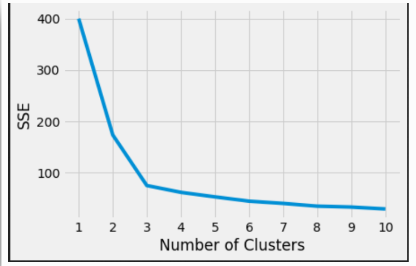
\includegraphics[width=0.45\textwidth]{img/img3.png}
                \caption{Grafico che mette in relazione k con gli errori quadratici.}
                \label{fig:un_agente}
            \end{figure}
            
            Possiamo notare che l'errore diminuisce drasticamente quando si passa da 2 a 3 cluster. L'errore diminuisce ancora man mano che si aumenta il numero di cluster ma con un \textit{k} troppo grande si ricade semplicemente in una situazione di overfitting. Il punto di gomito rappresenta l'ottimalità del compromesso fra numero di cluster ed errore quadratico. Nel caso in questione il valore ottimale è 3 o 4.
            
        \subsubsection{Coefficiente di forma, o Silhouette coefficient}
            Questo è una misura di coesione e separazione tra i dati. In particolare quantifica quanto i dati siano ben disposti nei cluster generati.
            
            Il coefficiente si basa su due dati: quanto bene sono \textit{ammassati} i dati nel cluster di riferimento, e quanto è distante ciascun campione da qualsiasi altro cluster, e il suo valore varia fra -1 e +1.
            
            Il coefficiente, per un punto i-esimo in un determinato cluster, è calcolato tramite la seguente formula:
            \begin{equation*}
                s(i) = \frac{b(i) - a(i)}{max(b(i),a(i))}    
            \end{equation*}
            
            con:
            \begin{itemize}
                \item $a(i)$ che rappresenta la distanza media dell'i-esimo punto rispetto a tutti gli altri punti appartenenti allo stesso cluster;
                
                \item $b(i)$ che rappresenta la distanza media dell’i-esimo punto rispetto a tutti gli altri punti appartenenti al cluster più vicino del cluster a cui è stato assegnato;
                
                \item $s(i)$ che rappresenta il coefficiente di silhouette dell’i-esimo punto.
            \end{itemize}
            
            Il valore finale di silhouette è dato dalla media dei coefficienti di silhouette calcolati per ogni elemento del problema.
            
        \subsubsection{MoJo distance}
            La Move-Join distance è una metrica che calcola il numero minimo di operazioni di spostamento e raggruppamento di elementi sono necessari per passare dal clustering identificato da un algoritmo al clustering ideale degli elementi.